\documentclass[10pt] {article}
\usepackage{fullpage}
\usepackage{amssymb}
\usepackage{graphicx}
\usepackage{amsthm}
\usepackage{hyperref}
\usepackage{amsmath}
\renewcommand\qedsymbol{$\blacksquare$}

\title{Homework 1 }
\author{Ricky Hempel}
\begin{document}
\maketitle
\begin{center}
0.1, 0.2, 0.3, 0.4, 0.5, 0.7, 0.8, 0.10, 0.12
\end{center}
\begin{enumerate}
\item[0.1]a. The set of all odd natural numbers.\\
b. The set of all even integers\\
c. The set of all even natural numbers\\
d. The set of all natural numbers, divisible by both 2 and 3 \\
e. The set of all strings comprising of 0's and 1's and every string is a palindrome. \\
f. The set of all integers that are equal to one added to that number.
\item[0.2]
a.$\{ 1,10,100 \}$\\
b.$\{x \mid x > 5$ for some x $\in \mathbb{Z} \}$\\
c.$\{1,2,3,4 \}$\\
d.$\{aba \}$\\
e.$\{ \varepsilon \}$\\
f.$\emptyset$
\item[0.3]
a.No.\\
b.Yes.\\
c.A $\cup$ B $= \{x,y,z\}$\\
d.A $\cap$ B $=\{ x,y\}$\\
e.A $\times$ B $= \{ (x,x),(x,y),(y,x),(y,y),(z,x),(z,y) \}$\\
f.\textit{P}(B)$= \{ \emptyset,\{x\},\{y\},\{x,y\} \}$
\item[0.4] A $\cdot$ B will have a $\cdot$ b number of elements in it. One of the methods of constructing the Cartesian products is to select an element of $A(x_a)$ and pair it with each and every element of B: $B(y_1,y_2,..y_b)$. This produces the pairings $\{(x_1,y_1),(x_2,y_2),...,(x_1,y_b) \}$. On repeating this procedure for each element $A(x_2)$ through $x_a$. First pairing will produce $$\sum_{i=1}^{n} (x_1,y_1) = a$$ pairs. As the iteration continues over the elements of A, a number of sets will get generated, each set having b pairs. Thus, the number of elements in A $\cdot$ B is a $\cdot$ b
\item[0.5] When the number of elements in the set S is n, then its power set consists of $2^{n}$ elements. The Power set is the set of all subset of the set S. The set C contains c elements such as $\{c_1 ,c_2, c_3,...,c_c\}$. Substituting, 'c' instead of 'n'. The number of elements in the power set of C is $2^c$ elements. 
\item[0.7] Let A$= \{1,2,3,4 \}$\\
a. The relation $R_1= \{(1,1),(2,2),(3,3),(4,4),(2,1),(1,2),(3,2),(2,3) \}$ is reflexive and symmetric, but not transitive\\
b. The relation $R_2= \{ (1,2),(2,1),(2,2),(1,1) \}$ is symmetric and transitive, but not reflexive. \\
c. The relation $R_3= \{ (1,2),(2,1) \}$ is symmetric, but neither reflexive nor transitive.
\item[0.8]
 \begin{figure}
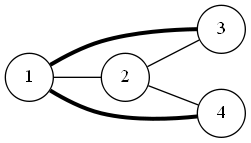
\includegraphics[width=0.5\textwidth]{8.png}
\caption{Graph for 0.8}
\label{8}
\end{figure} 
Nodes 1 and 2 have a degree of 3, and nodes 3 and 4 have a degree of 2. A path from 3 to 4 are the thick lines. Which starts at 3 goes to 1 and lastly ends at 4. 
\item[0.10]Let a$=$b$=$1
\begin{align*}
a&=b\\
a^{2}&=ab\\
a^{2}-b^{2}&=ab-b^{2}\\
(a+b)(a-b)&=b(a-b)\\
a+b&=b\\
2&=1\\
\end{align*}
The error happens when they divide (a-b) by (a-b). By substitution we get (1-1) which is zero divided by zero and we can not divide by zero, so this is where they go wrong and everything after this step is false.
\item[0.12] The proof fails at k$=$2 because $h_1$ and $h_2$ will be disjoint. Therefore, the induction step tells us only that each horse has the same color as itself. Consequently, we can not jump to the conclusion that the horses are the same color.
\end{enumerate}
\end{document}
